% Template for solutions write-ups, STAT 460/560
% Some basic notation is defined in 'macros/basic-math-macros'

\documentclass{article}
\usepackage{verbatim}
\usepackage{titlesec}

\def\coursename{STAT 447C: Bayesian Statistics}
\def\semester{Fall 2024}

\setlength{\oddsidemargin}{0.0 in}
\setlength{\evensidemargin}{0.0 in} 
\setlength{\topmargin}{-0.6 in} 
\setlength{\textwidth}{6.5 in} 
\setlength{\textheight}{8.5 in}
\setlength{\headsep}{0.75 in} 
\setlength{\parindent}{0 in}
\setlength{\parskip}{0.1 in}

\titleformat*{\section}{\Large\bfseries}


% prints box at top of first page with relevant info
\newcommand{\problemset}[3]{
   \pagestyle{myheadings}
   \thispagestyle{plain}
   \newpage
   \noindent
   \begin{center}
   \framebox{
      \vbox{\vspace{2mm}
    \hbox to 6.28in { {\bf \coursename
                        \hfill \semester} }
       \vspace{4mm}
       \hbox to 6.28in { {\Large \hfill #3  \hfill} }
       \vspace{2mm}
       \hbox to 6.28in { {\it #1 \hfill \texttt{#2}} }
      \vspace{2mm}}
   }
   \end{center}
   \vspace*{4mm}
}

\newcommand{\qsol}[1]{\section{#1}}
  % DO NOT CHANGE
% \usepackage{graphicx,amssymb,amsmath,amsthm,mathrsfs}
% \usepackage{multirow,makeidx,algorithmic,algorithm}
\usepackage{multirow,makeidx,algpseudocode,algorithm}
\usepackage{mathtools}
\usepackage{enumitem}
 
\usepackage{parskip}
\usepackage{setspace}
\usepackage{float, graphicx}
\usepackage{adjustbox}
\usepackage{bbm}
\usepackage{tabularx}
\usepackage{subfigure}
\usepackage{amsmath,amssymb,amsfonts,amsthm,amsbsy,amstext,mathrsfs}
\usepackage{hyperref}
\usepackage{url}
\usepackage{color}
\usepackage{graphicx} % Required for inserting images
\usepackage[utf8]{inputenc}

%% reference
\usepackage[round]{natbib}
\bibliographystyle{abbrvnat}
% \usepackage{cite}
% \bibliographystyle{plainurl}
% \bibliographystyle{abbrv}
% \bibliographystyle{plain}
% \bibliographystyle{unsrt}


%% code in-text
\usepackage{listings}
\usepackage{xcolor}

\definecolor{codegreen}{rgb}{0,0.6,0}
\definecolor{codegray}{rgb}{0.5,0.5,0.5}
\definecolor{codepurple}{rgb}{0.58,0,0.82}
\definecolor{backcolour}{rgb}{0.95,0.95,0.92}

\lstdefinestyle{mystyle}{
    backgroundcolor=\color{backcolour},   
    commentstyle=\color{codegreen},
    keywordstyle=\color{magenta},
    numberstyle=\tiny\color{codegray},
    stringstyle=\color{codepurple},
    basicstyle=\ttfamily\footnotesize,
    breakatwhitespace=false,         
    breaklines=true,                 
    captionpos=b,                    
    keepspaces=true,                 
    numbers=left,                    
    numbersep=5pt,                  
    showspaces=false,                
    showstringspaces=false,
    showtabs=false,                  
    tabsize=2
}

\lstset{style=mystyle}


%% layout
\oddsidemargin 3mm
\evensidemargin 3mm
\topmargin -12mm
\textheight 660pt
\textwidth 450pt  % DO NOT CHANGE
% ADD YOUR CUSTOM NOTATION HERE
\newcommand{\R}{\mathbb R}
\newcommand{\Z}{\mathbb Z}
\newcommand{\Q}{\mathbb Q}
\newcommand{\N}{\mathbb N}
\newcommand{\C}{\mathbb{C}}
\newcommand{\1}{\mathbbm{1}}
\newcommand{\E}{\mathbb E}
\newcommand{\Mcal}{{\cal M}}
\newcommand{\Ncal}{{\cal N}}
\newcommand{\Acal}{{\cal A}}
\newcommand{\Bcal}{{\cal B}}
\newcommand{\Fcal}{{\cal F}}
\newcommand{\Ecal}{{\cal E}}
\newcommand{\Gcal}{{\cal G}}
\newcommand{\Hcal}{{\cal H}}
\newcommand{\Scal}{{\cal S}}
\newcommand{\Xcal}{{\cal X}}
\newcommand{\Lcal}{{\cal L}}
\newcommand{\Mscr}{\mathscr{M}}
\newcommand{\eps}{\varepsilon}
\renewcommand{\P}{\mathbb P}
\DeclareMathOperator{\Var}{Var}
\DeclareMathOperator{\Poi}{Poi}
\DeclareMathOperator{\Cov}{Cov}
\DeclareMathOperator{\Exp}{Exp}
\DeclareMathOperator{\Bin}{Bin}
\DeclareMathOperator{\Geom}{Geom}
\DeclareMathOperator{\Unif}{Unif}
\DeclareMathOperator{\Bernoulli}{Bernoulli}
\DeclareMathOperator{\BetaMP}{BetaMP}
\DeclareMathOperator{\Beta}{Beta}
\newcommand{\abs}[1]{\left|#1\right|}
\newcommand{\norm}[1]{\left\lVert#1\right\rVert}
\newcommand{\floor}[1]{\lfloor#1\rfloor}
\newcommand{\ceil}[1]{\lceil#1\rceil}
\newcommand{\ds}{\displaystyle}
\newcommand{\inv}[1]{#1^{-1}}
\newcommand{\vect}[1]{\boldsymbol{#1}}
\DeclareMathOperator*{\argmax}{arg\,max}
\DeclareMathOperator*{\argmin}{arg\,min}
\newcommand{\convdist}[0]{\overset{d}{\longrightarrow}}
\newcommand{\convprob}[0]{\overset{p}{\longrightarrow}}
\newcommand{\convas}[0]{\overset{a.s.}{\longrightarrow}}
\newcommand{\partiald}[1]{\frac{\partial}{\partial{#1}}}
\newcommand{\partialdd}[1]{\frac{\partial^2}{\partial{#1^2}}}
% \newtheorem{definition}{Definition}[section]
% \newtheorem{theorem}{Theorem}[section]
% \newtheorem{corollary}{Corollary}[theorem]
% \newtheorem{lemma}{Lemma}[theorem]
% \newtheorem{proposition}[theorem]{Proposition}

\newtheorem{definition}{Definition}[section]
\newtheorem{theorem}{Theorem}[section]
\newtheorem{corollary}{Corollary}[section]
\newtheorem{lemma}{Lemma}[section]
\newtheorem{proposition}{Proposition}[section]
\newtheorem*{remark}{Remark}

\renewcommand{\algorithmicrequire}{ \textbf{Input:}} %Use Input in the format of Algorithm
\renewcommand{\algorithmicensure}{ \textbf{Output:}} %UseOutput in the format of Algorithm


%%
% full alphabets of different styles
%%

% bf series
\def\bfA{\mathbf{A}}
\def\bfB{\mathbf{B}}
\def\bfC{\mathbf{C}}
\def\bfD{\mathbf{D}}
\def\bfE{\mathbf{E}}
\def\bfF{\mathbf{F}}
\def\bfG{\mathbf{G}}
\def\bfH{\mathbf{H}}
\def\bfI{\mathbf{I}}
\def\bfJ{\mathbf{J}}
\def\bfK{\mathbf{K}}
\def\bfL{\mathbf{L}}
\def\bfM{\mathbf{M}}
\def\bfN{\mathbf{N}}
\def\bfO{\mathbf{O}}
\def\bfP{\mathbf{P}}
\def\bfQ{\mathbf{Q}}
\def\bfR{\mathbf{R}}
\def\bfS{\mathbf{S}}
\def\bfT{\mathbf{T}}
\def\bfU{\mathbf{U}}
\def\bfV{\mathbf{V}}
\def\bfW{\mathbf{W}}
\def\bfX{\mathbf{X}}
\def\bfY{\mathbf{Y}}
\def\bfZ{\mathbf{Z}}

% bb series
\def\bbA{\mathbb{A}}
\def\bbB{\mathbb{B}}
\def\bbC{\mathbb{C}}
\def\bbD{\mathbb{D}}
\def\bbE{\mathbb{E}}
\def\bbF{\mathbb{F}}
\def\bbG{\mathbb{G}}
\def\bbH{\mathbb{H}}
\def\bbI{\mathbb{I}}
\def\bbJ{\mathbb{J}}
\def\bbK{\mathbb{K}}
\def\bbL{\mathbb{L}}
\def\bbM{\mathbb{M}}
\def\bbN{\mathbb{N}}
\def\bbO{\mathbb{O}}
\def\bbP{\mathbb{P}}
\def\bbQ{\mathbb{Q}}
\def\bbR{\mathbb{R}}
\def\bbS{\mathbb{S}}
\def\bbT{\mathbb{T}}
\def\bbU{\mathbb{U}}
\def\bbV{\mathbb{V}}
\def\bbW{\mathbb{W}}
\def\bbX{\mathbb{X}}
\def\bbY{\mathbb{Y}}
\def\bbZ{\mathbb{Z}}

% cal series
\def\calA{\mathcal{A}}
\def\calB{\mathcal{B}}
\def\calC{\mathcal{C}}
\def\calD{\mathcal{D}}
\def\calE{\mathcal{E}}
\def\calF{\mathcal{F}}
\def\calG{\mathcal{G}}
\def\calH{\mathcal{H}}
\def\calI{\mathcal{I}}
\def\calJ{\mathcal{J}}
\def\calK{\mathcal{K}}
\def\calL{\mathcal{L}}
\def\calM{\mathcal{M}}
\def\calN{\mathcal{N}}
\def\calO{\mathcal{O}}
\def\calP{\mathcal{P}}
\def\calQ{\mathcal{Q}}
\def\calR{\mathcal{R}}
\def\calS{\mathcal{S}}
\def\calT{\mathcal{T}}
\def\calU{\mathcal{U}}
\def\calV{\mathcal{V}}
\def\calW{\mathcal{W}}
\def\calX{\mathcal{X}}
\def\calY{\mathcal{Y}}
\def\calZ{\mathcal{Z}}


%%%%%%%%%%%%%%%%%%%%%%%%%%%%%%%%%%%%%%%%%%%%%%%%%%%%%%%%%%
% text short-cuts
\def\iid{i.i.d.\ } %i.i.d.
\def\ie{i.e.\ }
\def\eg{e.g.\ }
\def\Polya{P\'{o}lya\ }
%%%%%%%%%%%%%%%%%%%%%%%%%%%%%%%%%%%%%%%%%%%%%%%%%%%%%%%%%%

% set theory/measure theory
\def\collection{\calC}
\newcommand{\sigalg}[1]{\mathcal{#1}}
\def\borel{\calB} %Borel sets
\def\sigAlg{\sigalg{H}} %sigma-algebra
\def\filtration{\calF} %filtration
\newcommand{\msblSpace}[1]{(#1,\sigalg{#1})}
\newcommand{\measSpace}[2][\mu]{(#2,\sigalg{#2},#1)}
\newcommand{\borelSpace}[1]{(#1,\borel(#1))}
\newcommand{\measFuncs}[1]{\sigalg{#1}^f}
\newcommand{\pbblSpace}{(\Omega,\sigAlg)}
\newcommand{\probSpace}[1][\bbP]{(\Omega,\sigAlg,#1)}

\def\leb{\lambda}

\def\finv{f^{-1}} % inverse
\def\ginv{g^{-1}} % inverse

% group theory
\def\grp{\calG} %group

% operators
\def\P{\bbP} %fundamental probability
\def\E{\bbE} %expectation
% conditional expectation
\DeclarePairedDelimiterX\bigCond[2]{[}{]}{#1 \;\delimsize\vert\; #2}
\newcommand{\conditional}[3][]{\bbE_{#1}\bigCond*{#2}{#3}}
\def\Law{\mathcal{L}} %law; this is by convention in the literature
% \def\indicator{\mathds{1}} % indicator function
\def\1{{\mathbf 1}}
\def\indicator{\1}

% binary relations
\def\condind{{\perp\!\!\!\perp}} %independence/conditional independence
\def\equdist{\stackrel{\text{\rm\tiny d}}{=}} %equal in distribution
\def\equas{\stackrel{\text{\rm\tiny a.s.}}{=}} %euqal amost surely
\def\simiid{\sim_{\mbox{\tiny iid}}} %sampled i.i.d

% common vectors and matrices
\def\onevec{\mathbf{1}}
\def\iden{\mathbf{I}} % identity matrix
\def\supp{\text{\rm supp}}

% misc
% floor and ceiling
% \DeclarePairedDelimiter{\ceilpair}{\lceil}{\rceil}
% \DeclarePairedDelimiter{\floor}{\lfloor}{\rfloor}
\newcommand{\argdot}{{\,\vcenter{\hbox{\tiny$\bullet$}}\,}} %generic argument dot
%%%%%%%%%%%%%%%%%%%%%%%%%%%%%%%%%%%%%%%%%%%%%%%%%%%%%%%%%%


 
\graphicspath{{./figures/}}







\begin{document}



% FILL IN:
%  - YOUR NAME, YOUR EMAIL (self-explanatory)
%  - The assignment number goes in ##
\problemset{Junsong Tang}{junsong.tang@stat.ubc.ca}{Exercise 8}



% WRITE YOUR SOLUTION TO THE FIRST QUESTION
\qsol{Calibration analysis via cross-validation}
\begin{enumerate}
\item 
Below is the Stan code for the ``hubble\_pred'' model:
\begin{lstlisting}[language=R]
  data {
    int<lower=0> N; // number of observations
    vector[N] xs;   // independent variable
    vector[N] ys;   // dependent variable
    real x_pred;  //independent variable for the left-out point
  }

  parameters {
    real slope;
    real<lower=0> sigma;
  }

  model {
    // prior
    slope ~ student_t(3, 0, 100);
    sigma ~ exponential(0.001);

    // likelihood
    ys ~ normal(slope*xs, sigma);
  }

  generated quantities {
    real y_pred = normal_rng(slope * x_pred, sigma); 
  }
\end{lstlisting}


\item 
\begin{lstlisting}[language=R]
  N_obs = nrow(df)
  N_train = N_obs-1
  train_test_dta = list(
      N  = N_train,
      xs = df$distance[-N_obs], 
      ys = df$velocity[-N_obs], 
      x_pred = df$distance[N_obs]
  )
  fit = sampling(stan_model("hubble_predict.stan"), 
  data=list(N=train_test_dta$N, ys=train_test_dta$ys, xs=train_test_dta$xs, x_pred=train_test_dta$x_pred), 
  iter=5000, control = list(max_treedepth = 15))

  quantile(extract(fit)$y_pred, prob=c(0.1, 0.9))
  # 0.485201900838154, 1.13324592497241
\end{lstlisting}
It can be seen that the leave-one-out $80\%$ credible interval for ``y\_pred'' quantity is: $[0.48, 1.14]$.

\item 
\begin{lstlisting}[language=R]
  # 3
  ci_limits = matrix(, nrow = N_obs, ncol = 2)
  for (i in (1:N_obs)) {
      trained = list(N=N_train, xs=df$distance[-i], ys=df$velocity[-i], x_pred=df$distance[i])
      fit_i = sampling(stan_model("hubble_predict.stan"), 
      data=list(N=trained$N, ys=trained$ys, xs=trained$xs, x_pred=trained$x_pred), 
      iter=5000, control = list(max_treedepth = 15))
      ci_limits[i,] = as.vector(quantile(extract(fit_i)$y_pred, prob=c(0.1, 0.9)))
  }
  merged_df = df %>% 
  bind_cols(data.frame(CI_L = ci_limits[,1], CI_R = ci_limits[,2])) %>% 
  mutate(Inside_CI = (velocity >= CI_L & velocity <= CI_R)) 
  merged_df %>% 
    ggplot(aes(x = 1:N_obs, y = velocity, ymin = CI_L, ymax = CI_R, color=Inside_CI)) +
    geom_point() + 
    geom_errorbar() +
    theme_minimal() +
    labs(x = "Point", y = "Velocity")
\end{lstlisting}
The plot of $80\%$ credible intervals for all observations are given as in Figure \ref{fig:ci}, hence it can be observed that the number of intervals that fail to capture the true points is $4$, so the proportion of such successful intervals is $\frac56 \approx 0.83$, which is similar to the nominal coverage level.
\begin{figure}[H]
  \centering
  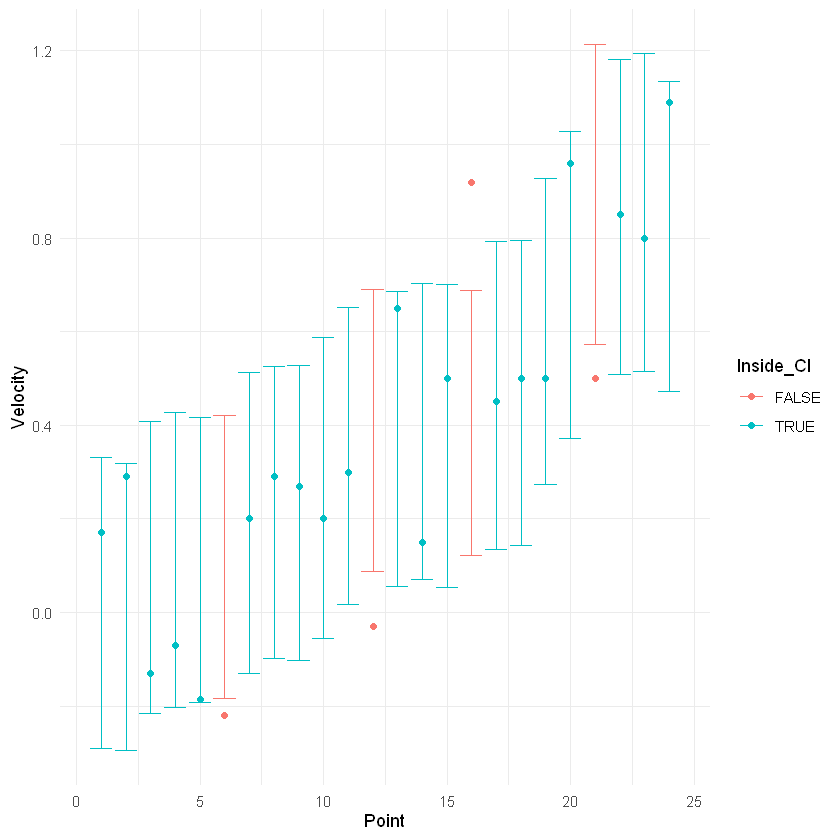
\includegraphics[width=0.8\textwidth, height=0.4\textheight]{ci.png}
  \caption{Plot of $80\%$ credible intervals for each observation}
  \label{fig:ci}
\end{figure}

\end{enumerate}



\qsol{Estimating asymptotic variance}
\begin{lstlisting}[language=R]
  # function
  estimate_asymptotic_variance = function(gamma, proposal_sd, C, S) {
    sum_E = 0
    sum_Ec_sq = 0
    init_so_far = numeric(C)
    counter = 0
    for (c in (1:C)) {    
        init_pt = rnorm(1, 0, 1)
        while (init_pt %in% init_so_far) {
            init_pt = rnorm(1, 0, 1)
        }
        counter = counter + 1
        init_so_far[counter] = init_pt
        E_c = mean(simple_mh(gamma, init_pt, S, proposal_sd))
        sum_E = sum_E + E_c * S
        sum_Ec_sq = sum_Ec_sq + E_c^2
    }
    return ((S/C)*sum_Ec_sq - S*(sum_E/(C*S))^2)
  }
\end{lstlisting}


\begin{lstlisting}[language=R]
  # generate the data frame for variances
  gamma = function(x) exp((-1/2)*x^2)
  proposal_sd_values = 2^seq(-10, 10, 1)
  n = length(proposal_sd_values)
  res = numeric(n)
  for (i in (1:n)) {
      res[i] = estimate_asymptotic_variance(gamma, proposal_sd_values[i], 100, 1000)
  }
  df = data.frame(estimated_mcmc_variance= res, proposal_sd = proposal_sd_values)

  # plot
  library(ggplot2)
  ggplot(df, aes(x = proposal_sd, y = estimated_mcmc_variance)) +
    geom_line() +
    geom_point() +
    scale_x_continuous(trans = "log2", breaks = proposal_sd_values) +
    labs(x = "Proposal SD (log2 scale)",
        y = "Estimated asymptotic variance",
        title = "Estimated asymptotic variance vs proposal SD") + 
    theme(axis.text.x = element_text(angle = 45, hjust = 1))
\end{lstlisting}

\begin{figure}[H]
\centering
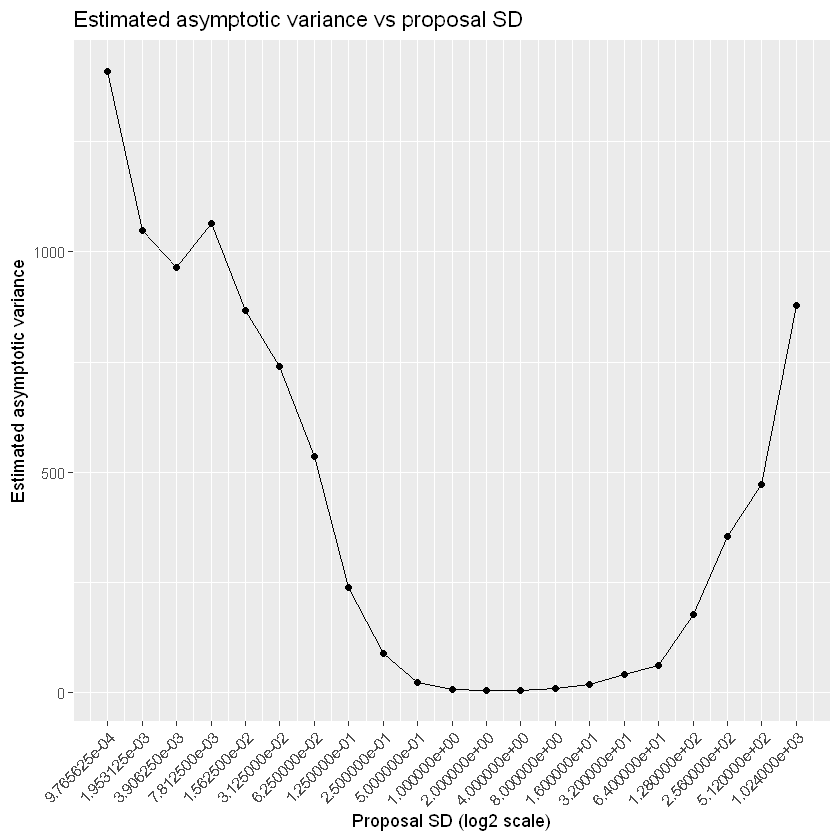
\includegraphics[width=0.8\textwidth, height=0.4\textheight]{est_var.png}
\caption{Plot of estimated variances of different proposal sd's}
\label{fig:est_var}
\end{figure}
From Figure \ref{fig:est_var}, it can be observed that if the proposal sd are in the range of $\{1, 2, 4\}$, then the estimated asymptotic variance seems to be optimal.

For $\gamma(x) = \exp(-\frac1{2000}x^2)$, since the standard deviation of the target increases, then the target is more spreaded. Using the optimal sd from above would cause the samples more concentrated at the initial point compared to the true target. So this will give a wrong estimation of the variance of target. While on the other side, for $\gamma(x) = \exp(-\frac{1}{2000}(x - 100)^2)$, because the target has the same variance as above but is merely shifted, so in this case, the optimal proposal sd will stay the same.
 
\end{document}

